% Copyright 2016 by Wang Kunzhen <wangkunzhen1993@gmail.com>.
%
% This is a latex template adapted from Till Tantau's Beamer template.
% It adds theme customizations for the convenience of users from the
% National University of Singapore. 
% 
% In principle, this file can be redistributed and/or modified under
% the terms of the GNU Public License, version 2.
%
% However, this file is supposed to be a template to be modified
% for your own needs. For this reason, if you use this file as a
% template and not specifically distribute it as part of a another
% package/program, I grant the extra permission to freely copy and
% modify this file as you see fit and even to delete this copyright
% notice. 

\documentclass[xcolor=dvipsnames]{beamer}

% There are many different themes available for Beamer. A comprehensive
% list with examples is given here:
% http://deic.uab.es/~iblanes/beamer_gallery/index_by_theme.html
% You can uncomment the themes below if you would like to use a different
% one:
%\usetheme{AnnArbor}
%\usetheme{Antibes}
%\usetheme{Bergen}
% \usetheme{Berkeley}
%\usetheme{Berlin}
%\usetheme{Boadilla}
% \usetheme{boxes}
%\usetheme{CambridgeUS}
%\usetheme{Copenhagen}
%\usetheme{Darmstadt}
%\usetheme{default}
%\usetheme{Frankfurt}
%\usetheme{Goettingen}
%\usetheme{Hannover}
% \usetheme{Ilmenau}
% \usetheme{JuanLesPins}
% \usetheme{Luebeck}
% \usetheme{Madrid}
\usetheme{Malmoe}
%\usetheme{Marburg}
% \usetheme{Montpellier}
% \usetheme{PaloAlto}
% \usetheme{Pittsburgh}
% \usetheme{Rochester}
% \usetheme{Singapore}
% \usetheme{Szeged}
% \usetheme{Warsaw}
\RequirePackage{amsmath}
\RequirePackage{mathtools}


\definecolor{nus-orange}{RGB}{239,124,0} 
\definecolor{nus-white}{RGB}{255,255,255}
\definecolor{nus-blue}{RGB}{0,61,124}
\definecolor{nus-black}{RGB}{0,0,0}

% Uncomment this section if you want the title background for each slide to be gradient like decaying from nus-orange to nus-white.
% \useoutertheme{shadow}
% \usepackage{tikz}
% \usetikzlibrary{shadings}
% \colorlet{titleleft}{nus-orange}
% \colorlet{titleright}{nus-orange!45!nus-white}
% \makeatletter
% \pgfdeclarehorizontalshading[titleleft,titleright]{beamer@frametitleshade}{\paperheight}{%
%   color(0pt)=(titleleft);
%   color(\paperwidth)=(titleright)}
% \makeatother
% End of gradient slide title effect.

\setbeamercolor{section in head/foot}{bg=nus-blue, fg=nus-white}
\setbeamercolor{subsection in head/foot}{bg=nus-blue, fg=nus-white}
\setbeamercolor{frametitle}{bg=nus-orange, fg=nus-black}
\setbeamercolor{title}{bg=nus-orange, fg=nus-white}
\setbeamercolor{alerted text}{fg=nus-orange}
\setbeamercolor{block title}{fg=nus-blue}
\setbeamercolor{block body}{fg=nus-black}

\setbeamertemplate{theorems}[numbered]
\setbeamertemplate{propositions}[numbered]

\setbeamertemplate{bibliography item}{\insertbiblabel}
\setbeamertemplate{title page}[default][colsep=-4bp,rounded=true, shadow=false]
\addtobeamertemplate{navigation symbols}{}{%
    \usebeamerfont{footline}%
    \usebeamercolor[fg]{footline}%
    \hspace{1em}%
    \insertframenumber/\inserttotalframenumber
}

\newcommand{\listofalgorithmes}{\tocfile{\listalgorithmcfname}{loa}}
\newcommand{\RR}{\mathbb{R}}
\newcommand{\xmin}{x_{\min}}
\newcommand{\GP}{\mathcal{GP}}
\newcommand{\N}{\mathcal{N}}
\newcommand{\D}{\mathcal{D}}
\newcommand{\y}{\mathbf{y}}
\newcommand{\ksi}{K+\sigma_n^2 I}
\newcommand{\X}{\mathcal{X}}
\newcommand{\G}{\mathcal{G}}
\newcommand{\inv}{^{\text{-}1}}
\newcommand{\ber}{\mathrm{Bernoulli}}
\newcommand{\ndim}{N_\mathrm{dim}}
\newcommand{\nsamples}{N_\mathrm{samples}}
\newcommand{\nparam}{N_\mathrm{param}}
\newcommand{\gs}{N_\mathrm{grid\_size}}
\newcommand{\nlvl}{N_\mathrm{lvl}}

\usepackage{tabularx} 
\usepackage{pifont}
\usepackage{amssymb}
\usepackage{algorithmic,float}
\usepackage[linesnumbered,ruled,vlined]{algorithm2e}
\usepackage{smartdiagram}
\smartdiagramset{%
set color list={gray,white,white,white,white,white}
}

\title{Configurable Vertically Split Neural Network}

\author{
  Han Liang Wee Eric (\texttt{A0065517A})\\
  \and
  Lok You Tan (\texttt{A0139248X})
}

\institute[National University of Singapore] % (optional, but mostly needed)
{
}

\titlegraphic{
   
\includegraphics[width=2cm]{NUS.pdf}
}

\date{AY2020/21 S1\\ Week 13}

% Uncomment this, if you want the table of contents to pop up at
% the beginning of each subsection:
% \AtBeginSubsection[]
% {
%   \begin{frame}<beamer>{Outline}
%     \tableofcontents[currentsection,currentsubsection]
%   \end{frame}
% }

\newcommand{\img}[2] {
  \begin{figure}
    \centering
    \includegraphics[height=#1\textheight]{images/#2}
  \end{figure}
}
\newcommand{\rimg}[2] {
  \begin{figure}
    \centering
    \includegraphics[height=#1\textheight]{../images/#2}
  \end{figure}
}
\newcommand{\inlineitem}{\leavevmode{\color{nus-blue}\usebeamertemplate{itemize item}} }

\begin{document}

\begin{frame}
  \titlepage
\end{frame}

\section{Introduction}
\begin{frame}{Split Neural Networks Learning in VFL}
  This project aims to implement a split learning approach of neural networks (NN) in VFL. Some
descriptions are as follows:
  \begin{enumerate}
    \item Code mainly in {\bf Python}, following Google Python style. Code {\bf sanity checks are needed}.
    \item Use Pytorch, Singa, or TensorFlow as local training framework. Define local training framework {\bf abstract} such that anyone can change it easily through configuration.
    \item Make each party’s local NN architecture {\bf configurable} such that the parties’ local model architectures can be different.
    \item Apply partially homomorphic encryption for {\bf secure aggregation} on the cut layer in the split learning approach.
  \end{enumerate}
\end{frame}

\subsection{Motivation}
\begin{frame}{Motivation}
  Premise
  \begin{itemize}
    \item Privacy laws (i.e. GDPR, CCPA) restrict entities from sharing data
  \end{itemize}
  Problem
  \begin{itemize}
      \item No longer able to use data from other entities. Model performance suffers
  \end{itemize}
  Need
  \begin{itemize}
      \item Distributed Secure Training - Training the AI models across `isolated islands'
    \item Data Privacy - Privacy must be preserved across nodes
  \end{itemize}
\end{frame}

\begin{frame}{Federated Learning and Split Learning}
    \begin{minipage}{.5\textwidth}
      \centering
      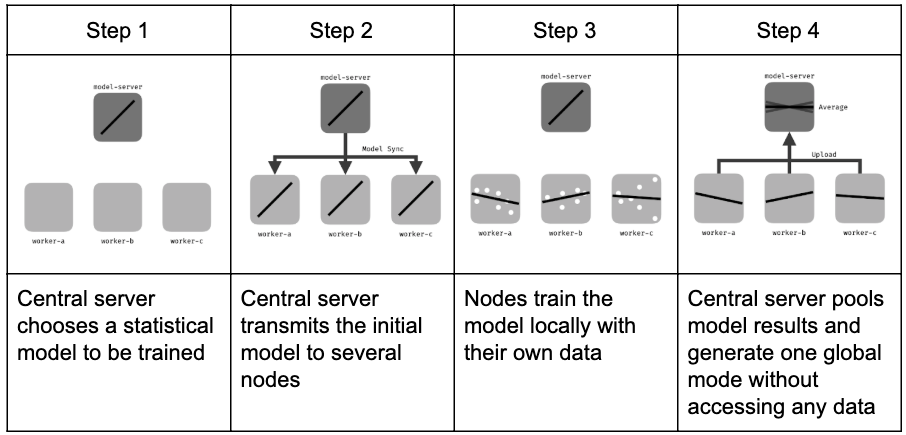
\includegraphics[width=1\linewidth]{images/federated.png}
      \label{fig:fed}
    \end{minipage}%
    \begin{minipage}{.5\textwidth}
      \centering
      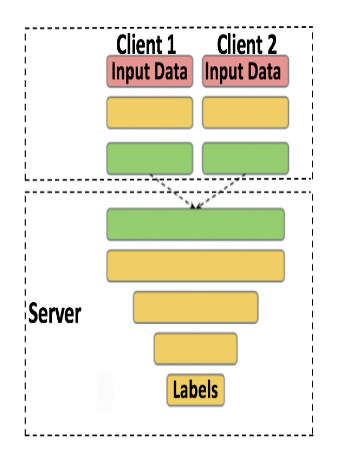
\includegraphics[width=0.8\linewidth]{images/split.png}
      \label{fig:split}
    \end{minipage}
    \footnotetext[1]{Diagram from \href{https://en.wikipedia.org/wiki/Federated\_learning}{https://en.wikipedia.org/wiki/Federated\_learning}}
    \footnotetext[2]{Diagram from \href{https://arxiv.org/pdf/1812.00564.pdf}{https://arxiv.org/pdf/1812.00564.pdf}}
\end{frame}

\begin{frame}{Data Leakage and Defenses}
    \begin{itemize}
        \item Recent works showed that sharing of gradients can result in data leakage 
        \begin{itemize}
            \item Deep leakage from gradients (Zhu et al.)
        \end{itemize}
    \end{itemize}
    Cryptographic defense measures
    \begin{itemize}
        \item Homomorphic encryption (slow)
        \item Secure aggregation (no need trusted third-party)
    \end{itemize}
    Desirable to have system that is configurable to cater to different needs and network architectures
\end{frame}

\subsection{Our contributions}
\begin{frame}{Our contributions}
  Key aspects:
  \begin{itemize}
    \item Implement a distributed VFL framework to train split NN
    \begin{itemize}
        \item Emphasis on configurability and flexibility
        \item Different parties can have different local model architectures
        \item User alignment using RSA blind signature-based private set intersection
    \end{itemize}
    \item Abstraction of underlying training framework
    \begin{itemize}
        \item Use of Pytorch
        \item Configuration file to unify different parties and their models
    \end{itemize}
    \item NN submodel configurable
    \begin{itemize}
      \item Pytorch load / save model state dictionary
      \item Expandable, with interface to load model via code
    \end{itemize}
    \item Secure aggregation on the cut layer
    \begin{itemize}
      \item Choice of Threshold-Paillier or SMPC
    \end{itemize}
  \end{itemize}
\end{frame}

\section{Our proposal}
\subsection{Methodology}
\begin{frame}{Assumptions}
  \begin{itemize}
      \item Semi-honest model (each party follows specified protocol exactly) that assumes there is a trusted party (Intel SGX)
      \item Labels {\it{Y}} held by one party (gradient computer)
      \item Rest are submodels
      \item No sharing of raw data or labels 
      \item Not all parties share same sample IDs (require user alignment)
  \end{itemize}
  No assumptions w.r.t network architecture / privacy techniques (e.g. homomorphic encryption, secure multi-party computation, differential privacy)\\
  System configurable and adaptable to different scenarios
\end{frame}

\begin{frame}{Local party training frameworks}
    Want flexibility for each party to use their own preferred ML framework
    \begin{itemize}
        \item Considered Tensorflow and Pytorch (two most popular frameworks)
    \end{itemize}
    Differences in gradient computation and backpropagation
    \begin{itemize}
        \item Tensorflow uses tf.GradientTape
        \item Pytorch uses backward()
    \end{itemize}
    Implementation for Tensorflow would be a lot more complicated (to be able to compute gradients, need to explicitly track outputs after they are sent to other parties)
    \begin{itemize}
        \item We picked Pytorch
    \end{itemize}
\end{frame}

\subsection{How we do it}
\begin{frame}{Wrapper}
    For the split / networking / encryption / related functionality, instead of implementing a custom layer, we use a wrapper because:
    \begin{itemize}
        \item Flexibility
        \item Ease of implementation
        \item Easily modified to accommodate additional ML frameworks / encryption / network protocols in the future
    \end{itemize}
\end{frame}

\begin{frame}{Configurability through YAML config}
    Configuration file to setup the entire network
    \begin{itemize}
        \item Trusted third party setups parties and starts training process using agreed-upon config file
        \item Each party free to have different local architectures as long as the aggregation is done properly
        \item Open and transparent contract 
    \end{itemize}
\end{frame}

\begin{frame}{YAML config}
    \img{0.85}{yaml2.png}
\end{frame}

\begin{frame}{Model definition}
    \begin{minipage}{.5\textwidth}
      \centering
      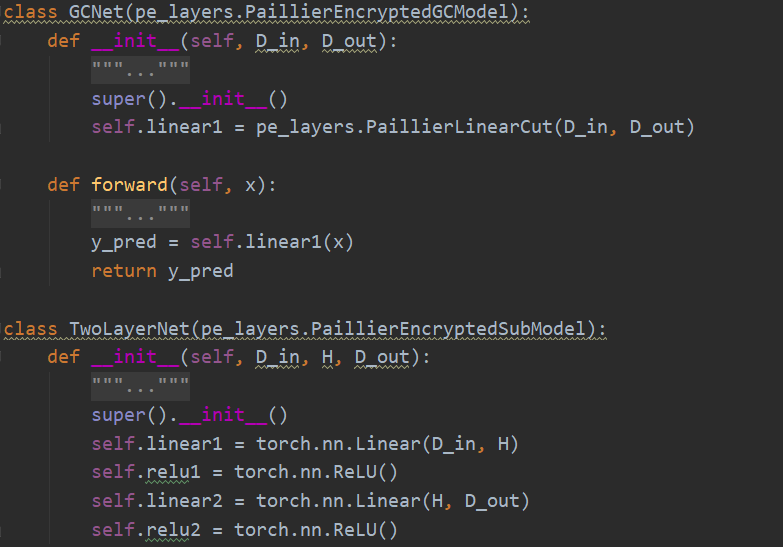
\includegraphics[width=1\linewidth]{images/gcnet.png}
      \label{fig:gcnet}
    \end{minipage}%
    \begin{minipage}{.5\textwidth}
      \centering
      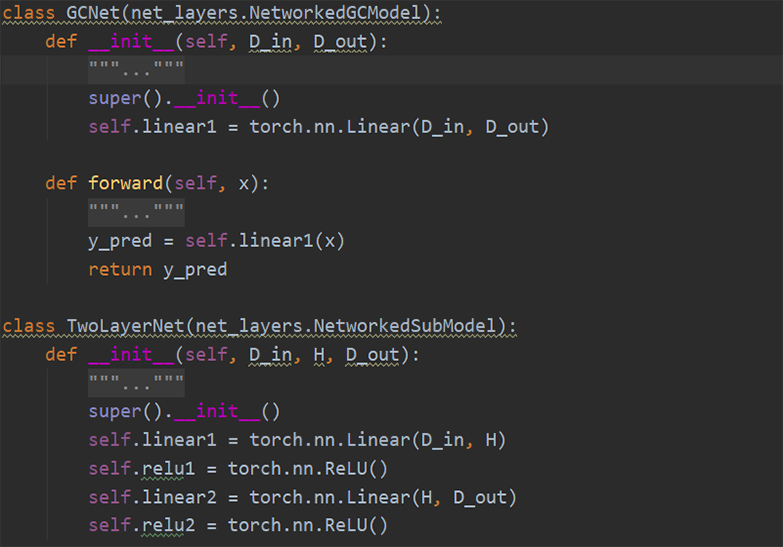
\includegraphics[width=1\linewidth]{images/unencryptedgcnet.png}
      \label{fig:unencryptedgcnet}
    \end{minipage}
\end{frame}

\begin{frame}{Architecture}
  \begin{itemize}
    \item {\bf GC}: Responsible for the labels and gradient propagation
    \item {\bf TP}: Defined in conjuction with the scenario
    \item {\bf Submodel}: Responsible for the sub neural network
  \end{itemize}
  Process:
  \begin{enumerate}
      \item Each party starts process
      \item Perform user alignment if necessary
      \item Setup individual networks on each party using YAML config
      \item Start training for \# of training iterations
          \begin{enumerate}
              \item Each \textbf{submodel} computes forward pass and passes to {\bf GC}
              \item {\bf GC} assembles received values from \textbf{submodel}s, computes forward pass and loss
              \item {\bf GC} backpropagates back to the \textbf{submodel}s
              \item {\bf Submodels} update their weights
          \end{enumerate}
  \end{enumerate}
\end{frame}

\begin{frame}{Our MNIST neural network}
\begin{minipage}{.3\textwidth}
  \centering
  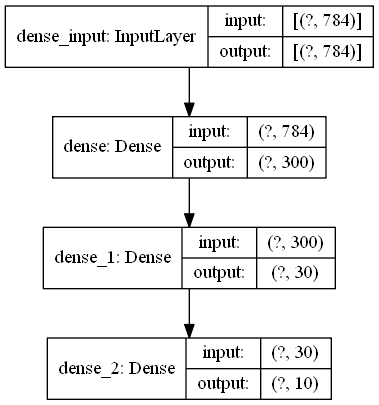
\includegraphics[width=1\linewidth]{images/combinedmodel.png}
  \label{fig:test1}
\end{minipage}%
\begin{minipage}{.7\textwidth}
  \centering
  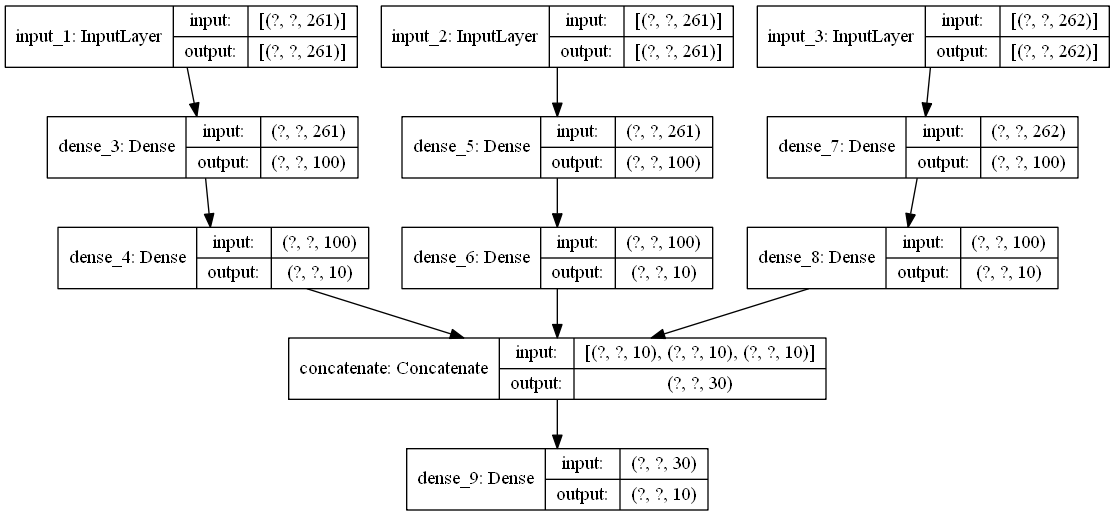
\includegraphics[width=1\linewidth]{images/splitmodel.png}
  \label{fig:test2}
\end{minipage}
\begin{itemize}
  \item Our neural network is exactly as defined by pytorch
  \item Custom defined cut layers can be defined (or not!)
\end{itemize}

\end{frame}

\begin{frame}{Different network architectures}
    Depending on the scenario, the cut layer will be different.
    \begin{center}
        \begin{tabularx}{\textwidth}{X X}
          Unencrypted & Paillier\\
          \img{0.5}{une.png}  & \img{0.5}{paillier.png} \\
        \end{tabularx}
    \end{center}
\end{frame}

\begin{frame}{Different network architectures}
  Depending on the scenario, the cut layer will be different.
  \begin{center}
      \begin{tabularx}{\textwidth}{X X}
        Threshold-Paillier & SMPC \\
        \img{0.5}{thres_paillier.png}  & \img{0.5}{smpc.png} \\
      \end{tabularx}
  \end{center}
\end{frame}


\begin{frame}{User alignment by private set intersection}
    Parties assumed not to share the same sample IDs (require user alignment)
    \\
    Private set intersection computes the intersection of sets of data without exposing them.
    \begin{itemize}
        \item Naive hashing (insecure against guessing attacks)
        \item Circuit-based (high comms, does not scale well)
        \item Public-key based (\textbf{RSA blind - linear complexity})
            \begin{itemize}
                \item widely available implementations
            \end{itemize}
        \item Oblivious transfer (current SOTA)
    \end{itemize}
    % https://eprint.iacr.org/2016/930.pdf
    2 kinds of PSI
    \begin{itemize}
        \item 2-party (Algorithm 1)
        \item multi-party
    \end{itemize}
\end{frame}

\begin{frame}{User alignment - general 2-party algorithm}
  \begin{algorithm}[H]
    \algsetup{linenosize=\tiny}
    \scriptsize
    \SetAlgoLined
    \SetKwInOut{Input}{input}
    \SetKwInOut{Output}{output}
    \Input{Node ID of the current node $n$ \newline
      Number of nodes in the network $N$ \newline
      Current node's address $h = H[n]$\newline
      Next node's address $h' = H[(n+1)\%N]$\newline
      Current node's database $D$}
    \Output{User aligned database $D$}
    \For{$i\in \left[0, N-1\right]$ \tcp*{Propagate $N-1$ times}}{
      \eIf{n == 0}{
        Update $D=$ Align-To($h'$, D)\tcp*{Update using $h'$}
        Align-From($D$)\tcp*{Wait for the previous node}
      }{
        Align-From($D$)\;
        Update $D=$ Align-To($h'$, D)\;
      }
    }
    \Return D\;
  \caption{User-Align}
  \end{algorithm}
\end{frame}

\begin{frame}{Different privacy techniques}
We are aiming to secure matrix multiplication (Linear layer $X\times W$) inside our cut layer.
Using our framework, we can use:
\begin{itemize}
    \item \textbf{Partially Homomorphic Encryption}
        \begin{itemize}
            \item \textbf{Paillier (server-client) [pe]}
            \item \textbf{Threshold-Paillier (distributed) [tpe]}
            \item Other additively homomorphic encryption schemes
        \end{itemize}
    \item \textbf{Secure multi-party computation [smpc]}
\end{itemize}
We implemented the items in \textbf{bold} and tested in our experiments.
We also define \textbf{TP} here together with the privacy technique.
We also implemented \textbf{Unsecure Cut Layer [une]} as a baseline.
\end{frame}

\begin{frame}{Partially homomorphic encryption - Paillier}
Implementation from \textit{phe} library
\begin{enumerate}
    \item Each \textbf{submodel} encrypts forward values using Paillier and sends results to \textbf{GC}
    \item Within the cut layer, \textbf{GC} does matrix multiplication before sending to \textbf{TP}
    \item \textbf{TP} decrypts, sends back to \textbf{GC} and training continues
    \item Equivalent process happens in the backward pass
\end{enumerate}
\textbf{TP}: Distribute keys, performs decryption
\end{frame}

%  Such an adversary controls one of the parties (statically, and so at the onsetof the computation) and follows the protocol specification exactly.  However, it may try to learnmore  information  than allowed by  looking  at the  transcript of  messages that  it received and itsinternal state.  Note that this is a very weak adversary model; if the adversary does anything notaccording to specificatiore– even just choosing its random tape in a non-random way – l (and there are actuaexamples of natural protocols withthis property).  Nevertheless, a protocol that is secure in the presence of semi-honest adversariesdoes  guarantee  that  there  is  noinadvertent  leakageof  information;  when  the  parties  involvedessentially trust each other butreant to make sure that no record of their input is found elsewhere,t are secure foemi-honest adversaries are oftendesigned as the first step towards achieving stronger notions of security

\begin{frame}{Partially homomorphic encryption - Threshold-Paillier}
Modified by us to work with Pytorch (threshold we use is all \textbf{submodel}s)
\begin{enumerate}
    \item Each \textbf{submodel} encrypts forward values using Paillier and sends results to \textbf{GC}
    \item Within the cut layer, \textbf{GC} does matrix multiplication and sends parts to \textbf{submodel}s
    \item Submodels decrypt and send each part back to \textbf{GC}
    \item \textbf{GC} assembles results and continues training
    \item Equivalent process happens in the backward pass.
\end{enumerate}
\textbf{TP}: Distribute keys
\end{frame}

\begin{frame}{Secure multi-party computation}
Implementation from \textit{PySyft}. Currently computed with only 2 \textbf{submodel}s (limitation of \textit{PySyft}).
\begin{enumerate}
    \item Matrix multiplication done in distributed manner
    \item Secret shares distributed 
    \item \textbf{GC} sends weights to \textbf{submodel}s
    \item Submodels do matrix multiplication and sends results to \textbf{GC}
    \item \textbf{GC} assembles them, and continues training
\end{enumerate}
\textbf{TP}: Not needed
\end{frame}

\begin{frame}{Other Engineering Details}
  Some additional features:
  \begin{itemize}
    \item SSL encryption is used between any communication
    \item Websockets are used
    \item Large data is batched when sent over the network
    \item User alignment can be done seprately
    \item Implemented a facility to checkpoint the training (but not fully implemented)
    \item We can easily convert our model to a pytorch model \textbf{[une-pytorch]}
    \item We can also run our model locally without network \textbf{[une-framework]}
  \end{itemize}
\end{frame}

\section{Experiments}

\subsection{Experiments}
\begin{frame}{Experiments and datasets}
    Experiment Setup: 
    \begin{itemize}
        \item Hardware: GCP VMs (e2-standard-4, e2-medium, e2-medium)
        \item Software: Conda, Python 3, \href{http://34.67.88.74:5000/mlflow/}{\underline{Mlflow}}
        \item Expt: Take the average of 3 runs, splits are done as per dataset
        \item Aim 1: Understand system behavior and performance behavior
        \begin{itemize}
            \item User alignment overhead
            \item System overhead
        \end{itemize}
        \item Aim 2: Show real-world application of our system
    \end{itemize}
    Datasets:
    \begin{itemize}
        \item \href{http://yann.lecun.com/exdb/mnist/}{\underline{MNIST handwritten digits}} - multi-class (0 to 9) 
        \item \href{https://www.kaggle.com/mlg-ulb/creditcardfraud}{\underline{Credit card fraud detection}} - binary classification of anonymized credit card transactions as genuine or fraudulent
    \end{itemize}
\end{frame}

\subsection{Metrics}
\begin{frame}{Metrics}
System overhead and real-world application
  \begin{itemize}
      \item Cross-entropy loss
      \item Test Accuracy / AUC-ROC (TPR against FPR. For unbalanced datasets - cc fraud. Higher is better)
      
      \begin{table}[]
        \centering
        \label{tab:my-table}
        \begin{tabular}{|l|l|}
        \hline
         & \# samples \\ \hline
        Genuine & 284315 \\ \hline
        Fraudulent & 492 \\ \hline
        \end{tabular}
        \end{table}
      \item Time taken to train
  \end{itemize}

User alignment overhead
  \begin{itemize}
      \item Time
      \item Communication costs (data transferred / received)
  \end{itemize}
\end{frame}

\subsection{Results}
\begin{frame}{User alignment overhead (MNIST)}
    \begin{minipage}{.5\textwidth}
      \centering
      \rimg{0.45}{ua_bytes.pdf}
    \end{minipage}%
    \begin{minipage}{.5\textwidth}
      \centering
      \rimg{0.45}{ua_time.pdf}
    \end{minipage}
    \begin{itemize}
      \item RSA PSI algorithm takes quite some time to run
      \item Possible to use a multi-party algorithm to replace this to improve efficiency
    \end{itemize}
\end{frame}

\begin{frame}{System overhead (MNIST)}
    \begin{minipage}{.5\textwidth}
      \centering
      \rimg{0.45}{mnist_accuracy.pdf}
    \end{minipage}%
    \begin{minipage}{.5\textwidth}
      \centering
      \rimg{0.45}{mnist_time.pdf}
    \end{minipage}
    \begin{itemize}
      \item Accuracy differences are due to the noise introduced
      \item Differences show the various inefficiencies
      \item Interestingly, une-framework is faster than pytorch (parallel)
    \end{itemize}
\end{frame}

\begin{frame}{Real-world application (credit card fraud detection)}
  \begin{minipage}{.6\textwidth}
    \centering
    \rimg{0.5}{ccfraud_roc_auc_score.pdf}
  \end{minipage}%
  \begin{minipage}{.4\textwidth}
    Features are PCA transformed into $30$ features.
    \begin{itemize}
      \item ROC AUC, higher is better
      \item Motivates our VFL framework
      \item Works as expected on Real-world dataset
      \item \emph{PS. we did not change any code.}
    \end{itemize}
  \end{minipage}
  
\end{frame}

\section{Conclusion}
\subsection{Our accomplishments}
\begin{frame}{Our accomplishments}
  \begin{itemize}
    \item Code mainly in {\bf Python}, following Google Python style. Code sanity checks are needed.
        \begin{itemize}
            \item [\checkmark] Python, unit tests (Threshold-Paillier, key serialization, user alignment, expt using baselines)
        \end{itemize}
    \item Use Pytorch, Singa, or TensorFlow as local training framework. Define local training framework abstract such that anyone can change it easily through configuration.
        \begin{itemize}
            \item [\checkmark] Pytorch (with ability to extend to other frameworks)
        \end{itemize}
    \item Make each party’s local NN architecture configurable such that the parties’ local model architectures can be different.
        \begin{itemize}
            \item [\checkmark] Configurable through YAML, flexible network architectures
        \end{itemize}
    \item Apply partially homomorphic encryption for {\bf secure aggregation} on the cut layer in the split learning approach.
        \begin{itemize}
            \item [\checkmark] Supports \emph{both} Paillier, Threshold-Paillier
        \end{itemize}
  \end{itemize}
\end{frame}

\begin{frame}{Conclusion - Final Thoughts}
  Went above and beyond:
  \begin{itemize}
    \item Demonstrate Cut-Layer configurablity - implementing Secure multi-party computation \& Threshold-Paillier (P2P)
    \item Demonstrate ability to swap out user alignment algorithms
    \item Implemented RSA-PSI algorithm
    \item Configurability in pytorch/yaml: load or not load statedict
    \item Extensive analysis of our UA and system performance
  \end{itemize}
  Takeaways: Homomorphic Encryption is not ready, more can be done. 
  Generally the field of privacy has active interest (ie. PySyft).
\end{frame}

\end{document}
